% =================================================================================================
% File:			client_tier/model/services.tex
% Description:	Defiinisce la sezione relativa al front-end dell'applicazione
% Created:		2015-04-10
% Author:		Tesser Paolo
% Email:		tesser.paolo@mashup-unipd.it
% =================================================================================================
% Modification History:
% Version		Modifier Date		Change											Author
% 0.0.1 		2015-04-10 			creato scheletro								Tesser Paolo
% =================================================================================================
%
%

% CONTENUTO DEL CAPITOLO
%

\subsubsection{client::model::services} % (fold)
\label{ssub:bdsm_app_client_model_services}
\begin{figure}[htbp]
	\centering
	\centerline{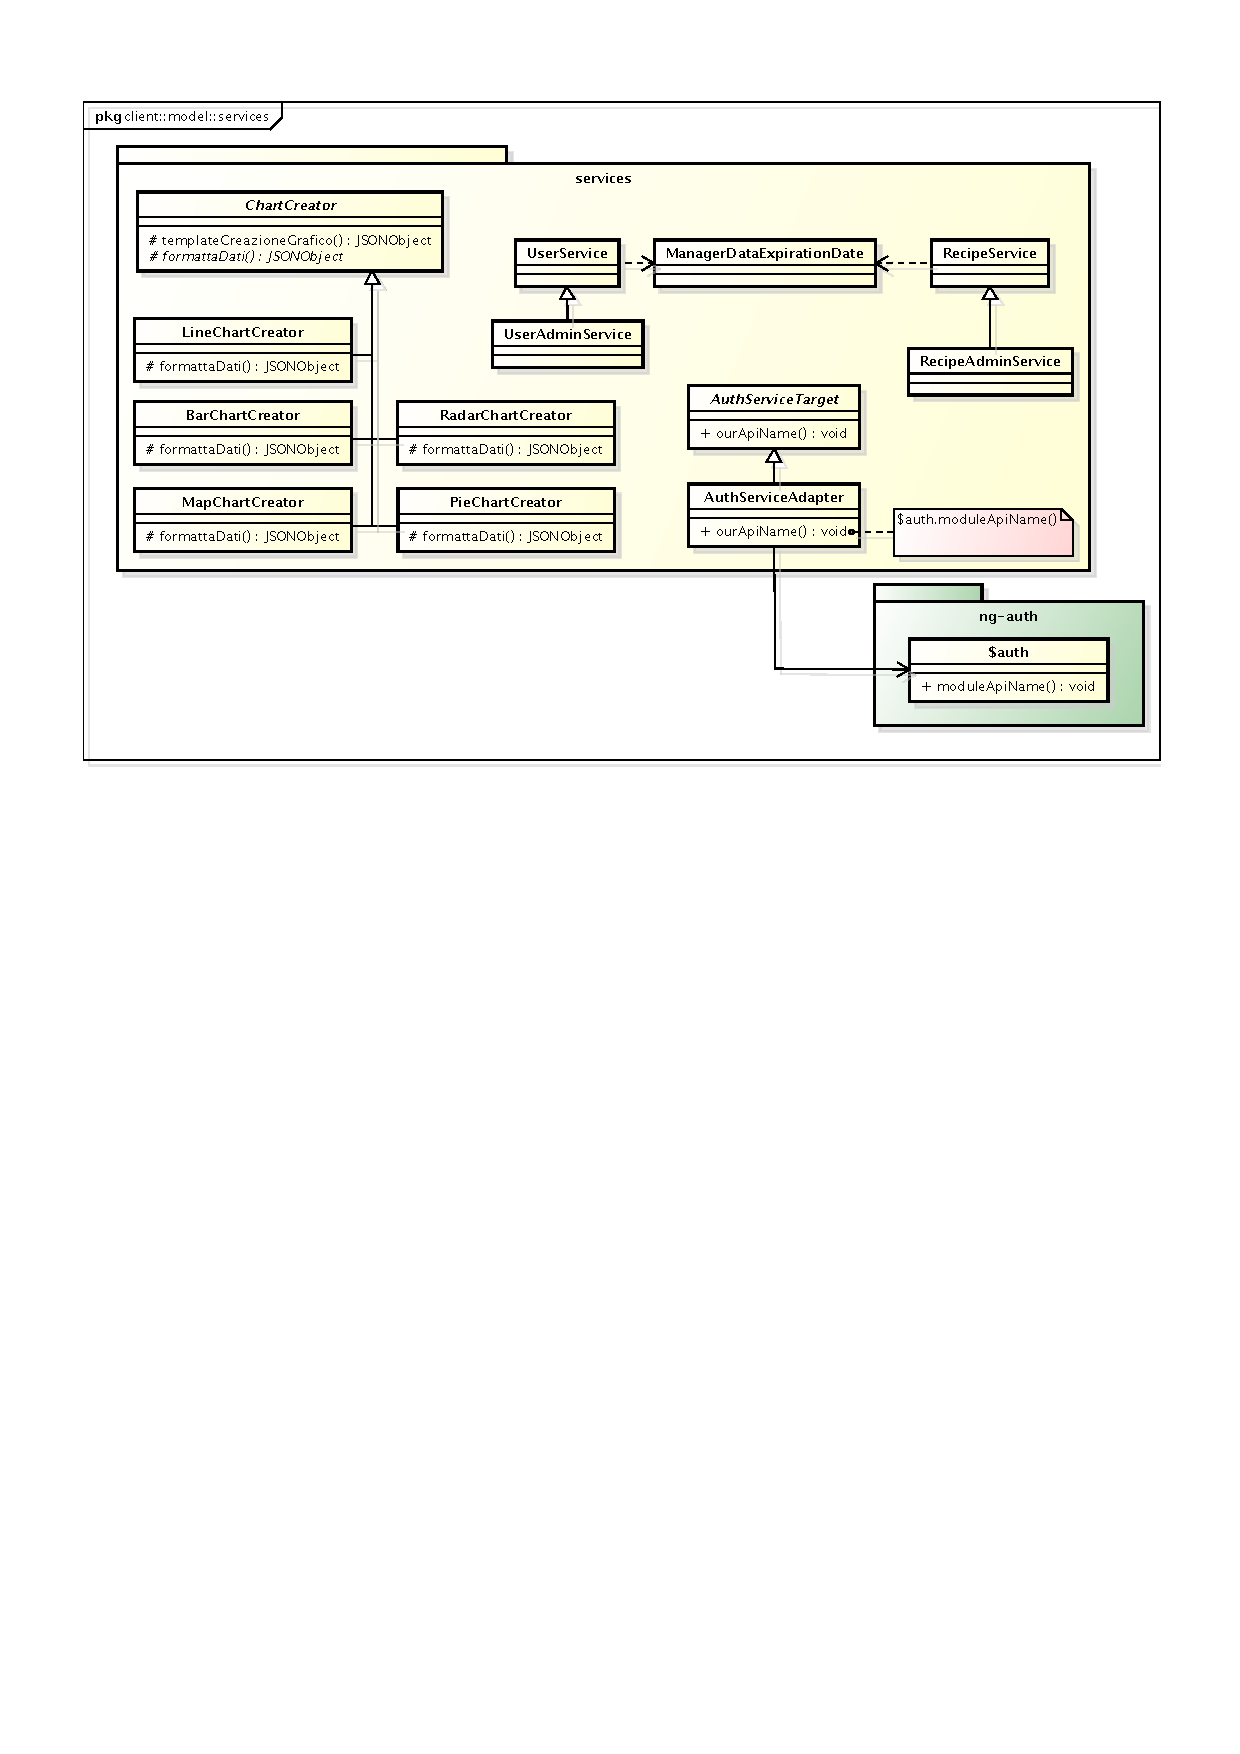
\includegraphics[scale=1.03]{./images/client/client_model_services.pdf}}
	\caption{Package - client::model}
\end{figure}

\begin{itemize}
	\item \textbf{Descrizione}: è il package che contiene le classi che sviluppano il core business dell'applicazione: in particolare gestiscono il recupero dei dati, siano essi salvati in locale o da recuperare chiamando il server, la creazione dei grafici e l'autenticazione. Tutte le classi contenute in questo package implementano il pattern \emph{Singleton};
	\item \textbf{Padre}: client::model
	\item \textbf{Interazione con altri componenti}:
		\begin{itemize}
			\item client::model::data
			\item client::controller
		\end{itemize}
\end{itemize}

	\paragraph{Classi} % (fold)

		\subparagraph{client::model::services::AuthServiceTarget} % (fold)
		\label{subp:client_model_services_authservice}
			\begin{itemize}
				\item \textbf{Descrizione}: è la classe di interfaccia per gestire le chiamate al modulo esterno usato per gestire l'autenticazione secondo il pattern \emph{Adapter} ;
				\item \textbf{Utilizzo}: Questa classe non è stata implementata in quanto non esistono interfacce in JavaScript, e grazie alla Dependency Injection è stato  possibile iniettare direttamente la classe AuthServiceAdapter dove è stato necessario.
			\end{itemize}
		% subparagraph client_model_services_authservicetarget (end)

		\subparagraph{client::model::services::AuthServiceAdapter} % (fold)
		\label{subp:client_model_services_authservice}
		\begin{figure}[htbp]
				\centering
				\centerline{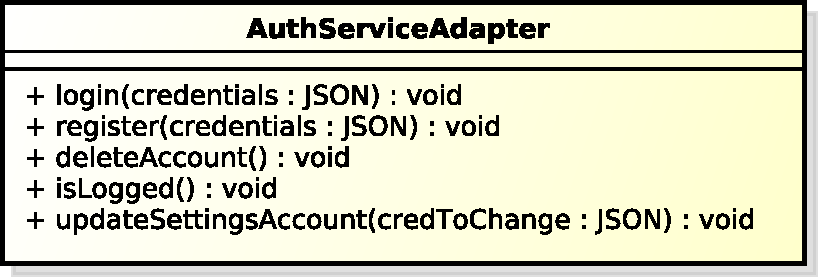
\includegraphics[scale=0.7]{./images/client/classes/model/auth_service_adapter.pdf}}
				\caption{Classe - client::model::services::RadarChartCreator}
			\end{figure}
			\begin{itemize}
				\item \textbf{Descrizione}: è la classe \emph{Adapter} che permette di invocare i metodi del modulo di autenticazione esterno invocando i metodi come presentati in AuthServiceTarget;
				\item \textbf{Utilizzo}:  i metodi di questa classe saranno invocati quando un utente effettua la registrazione al servizio o effettua un login/logout. Questa classe è stata implementata col nome più semplice di AuthService in quanto non è necessario distinguerla dalla classe Target (non implementata);
				\item \textbf{Relazioni con altre classi}:
					\begin{itemize}
						\item client::controller::public::LoginCtrl
						\item client::controller::public::RegisterCtrl
						\item client::controller::user::LogoutCtrl
						\item ng-auth::\$auth
					\end{itemize}
				\item \textbf{Attributi}: N/A
				\item \textbf{Metodi}:
				\begin{itemize}
					\item \textcolor{forestgreen}{\texttt{+ login(credentials)}}
					\begin{description}
						\item \textbf{Descrizione}: metodo per effettuare il login. Invia al server il JSON credentials, nella forma:
								\begin{verbatim}
									{
									    email: "info@mashup-unipd.it",
									    pwd: 'password'
									}
								\end{verbatim}  
					\end{description}
					\item \textcolor{forestgreen}{\texttt{+ register(credentials)}}
					\begin{description}
						\item \textbf{Descrizione}: metodo per effettuare la registrazione. Invia al server il JSON credentials, nella forma:
								\begin{verbatim}
									{
									    username: "MashUp",
									    email: "info@mashup-unipd.it",
									    pwd: 'password'
									}
								\end{verbatim}  
					\end{description}
					\item \textcolor{forestgreen}{\texttt{+ deleteAccount()}}
					\begin{description}
						\item \textbf{Descrizione}: metodo per eliminare l'account che invia la richiesta al server. 
					\end{description}
					\item \textcolor{forestgreen}{\texttt{+ isLogged()}}
					\begin{description}
						\item \textbf{Descrizione}: metodo che restituisce un booleano true se l'utente è autenticato al servizio.
					\end{description}
					\item \textcolor{forestgreen}{\texttt{+ updateSettingsAccount(credToChange)}}
					\begin{description}
						\item \textbf{Descrizione}: metodo per cambiare le proprie credenziali. Invia al server un JSON nella forma seguente:
								\begin{verbatim}
									{
									    username: "MashUp",
									    email: "info@mashup-unipd.it",
									    pwd: 'password'
									}
								\end{verbatim}  
					\end{description}
				\end{itemize}	
			\end{itemize}
		% subparagraph client_model_services_authserviceadapter (end)


		\subparagraph{client::model::services::RecipeService} % (fold)
		\label{subp:client_model_services_recipeservice}
		\begin{figure}[htbp]
				\centering
				\centerline{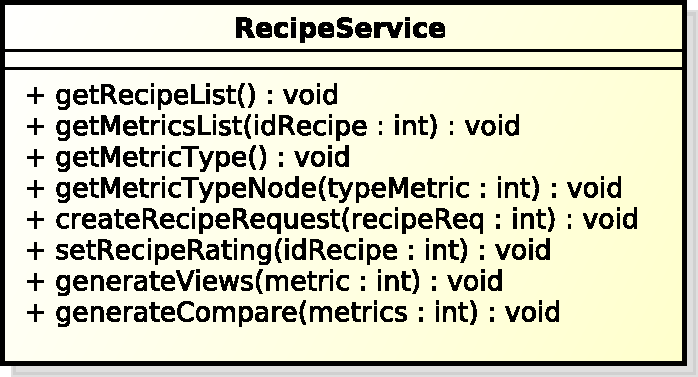
\includegraphics[scale=0.7]{./images/client/classes/model/recipe_service.pdf}}
				\caption{Classe - client::model::services::RadarChartCreator}
			\end{figure}
			\begin{itemize}
				\item \textbf{Descrizione}: è la classe che racchiude i metodi per reperire i dati relativi alle Recipe, siano essi salvati in locale o da recuperare dal server, inoltre gestisce l'invio di richieste di Recipe al server;
				\item \textbf{Utilizzo}: i suoi metodi vengono invocati ogni volta che sia necessario avere dei dati relativi a una o più Recipe per un utente non amministratore, o se un utente non amministratore desidera inviare una richiesta di Recipe;
				\item \textbf{Relazioni con altre classi}:
					\begin{itemize}
						\item client::model::data::RecipeRequestModel
						\item client::model::services::ManagerDataExpirationDate
						\item client::controller::user::RecipeCtrl
						\item client::controller::user::MetricsCtrl
						\item client::controller::user::ChartsCtrl
						\item client::controller::user::CompareCtrl
					\end{itemize}
				\item \textbf{Attributi}: N/A
				\item \textbf{Metodi}:
				\begin{itemize}
					\item \textcolor{forestgreen}{\texttt{+ getRecipeList()}}
					\begin{description}
						\item \textbf{Descrizione}: metodo per ottenere la lista delle recipe disponibili. 
					\end{description}
					\item \textcolor{forestgreen}{\texttt{+ getMetricsList(idRecipe)}}
					\begin{description}
						\item \textbf{Descrizione}: metodo per ottenere la lista delle metriche dato l'id di una recipe.
					\end{description}
					\item \textcolor{forestgreen}{\texttt{+ getMetricType()}}
					\begin{description}
						\item \textbf{Descrizione}: metodo che restituisce la lista delle categorie presenti (i vari social). 
					\end{description}
					\item \textcolor{forestgreen}{\texttt{+ getMetricTypeNode(typeMetric)}}
					\begin{description}
						\item \textbf{Descrizione}: metodo che la lista dei tipi di metriche data la categoria.
					\end{description}
					\item \textcolor{forestgreen}{\texttt{+ createRecipeRequest(recipeReq)}}
					\begin{description}
						\item \textbf{Descrizione}: metodo per inviare una nuova richiesta di ricetta. Invia un JSON nella forma descritta dalla classe RecipeRequestModel.
					\end{description}
					\item \textcolor{forestgreen}{\texttt{+ setRecipeRating(idRecipe)}}
					\begin{description}
						\item \textbf{Descrizione}: metodo per impostare un rating a una recipe e inviare il voto al server.
					\end{description}
					\item \textcolor{forestgreen}{\texttt{+ generateViews(metric)}}
					\begin{description}
						\item \textbf{Descrizione}: metodo che data una metrica (nel formato descritto da MetricModel) restituisce l'html per generare i grafici associati a quella metrica. 
					\end{description}
					\item \textcolor{forestgreen}{\texttt{+ generateCompare(metrics)}}
					\begin{description}
						\item \textbf{Descrizione}: metodo che dato un array di metriche (nel formato descritto da MetricModel) restituisce l'html per generare i grafici di confronto di quelle metriche. 
					\end{description}
				\end{itemize}	
			\end{itemize}
		% subparagraph client_model_services_recipeservice (end)

		\subparagraph{client::model::services::RecipeAdminService} % (fold)
		\label{subp:client_model_services_recipeadminservice}
		\begin{figure}[htbp]
				\centering
				\centerline{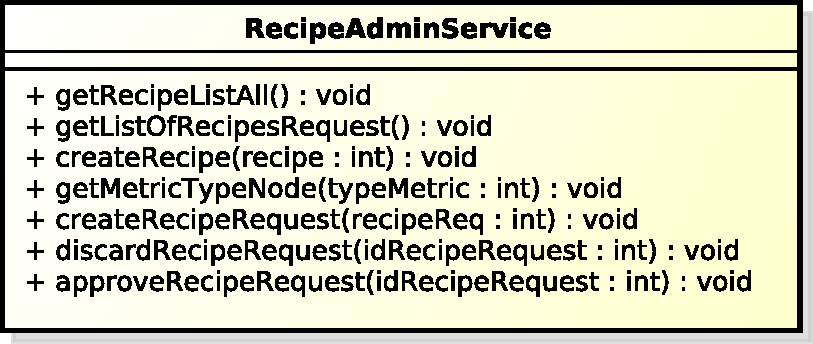
\includegraphics[scale=0.7]{./images/client/classes/model/recipe_admin_service.pdf}}
				\caption{Classe - client::model::services::RadarChartCreator}
			\end{figure}
			\begin{itemize}
				\item \textbf{Descrizione}: è la classe che oltre a gestire ciò che è gestito dalla classe padre si occupa dell'inserimento di nuove recipe nel server e dell'eliminazione di Recipe già presenti;
				\item \textbf{Utilizzo}: i suoi metodi vengono invocati quando un utente amministratore desidera agire su dati di Recipe da pagine non accessibili a un utente non amministratore;
				\item \textbf{Classi ereditate}:
					\begin{itemize}
						\item client::model::services::RecipeService
					\end{itemize}
				\item \textbf{Relazioni con altre classi}:
					\begin{itemize}
						\item client::model::data::RecipeInsertModel
						\item client::model::services::ManagerDataExpirationDate
						\item client::controller::admin::RecipeConfigCtrl
						\item client::controller::admin::InsertRecipeCtrl
					\end{itemize}
				\item \textbf{Attributi}: N/A
				\item \textbf{Metodi}:
				\begin{itemize}
					\item \textcolor{forestgreen}{\texttt{+ getRecipeListAll()}}
					\begin{description}
						\item \textbf{Descrizione}: metodo per ottenere la lista delle recipe disponibili con tutti i dati ad esse associate (inclusi i ratings). 
					\end{description}
					\item \textcolor{forestgreen}{\texttt{+ getListOfRecipesRequest()}}
					\begin{description}
						\item \textbf{Descrizione}: metodo per ottenere la lista delle richieste di recipe.
					\end{description}
					\item \textcolor{forestgreen}{\texttt{+ createRecipe(recipe)}}
					\begin{description}
						\item \textbf{Descrizione}: metodo per aggiungere una ricetta al sistema (l'argomento è nella forma descritta da RecipeModel). 
					\end{description}
					\item \textcolor{forestgreen}{\texttt{+ getMetricTypeNode(typeMetric)}}
					\begin{description}
						\item \textbf{Descrizione}: metodo che la lista dei tipi di metriche data la categoria.
					\end{description}
					\item \textcolor{forestgreen}{\texttt{+ createRecipeRequest(recipeReq)}}
					\begin{description}
						\item \textbf{Descrizione}: metodo per inviare una nuova richiesta di ricetta. Invia un JSON nella forma descritta dalla classe RecipeRequestModel.
					\end{description}
					\item \textcolor{forestgreen}{\texttt{+ discardRecipeRequest(idRecipeRequest)}}
					\begin{description}
						\item \textbf{Descrizione}: metodo che elimina una richiesta di Recipe (dato il suo id). 
					\end{description}
					\item \textcolor{forestgreen}{\texttt{+ approveRecipeRequest(idRecipeRequest)}}
					\begin{description}
						\item \textbf{Descrizione}: metodo che genera una Recipe come descritta da una richiesta di recipe (di cui è dato l'id), eliminando poi quella richiesta.
					\end{description}
				\end{itemize}
			\end{itemize}
		% subparagraph client_model_services_recipeadminservice (end)


		\subparagraph{client::model::services::UserService} % (fold)
		\label{subp:client_model_services_userservice}
		\begin{figure}[htbp]
				\centering
				\centerline{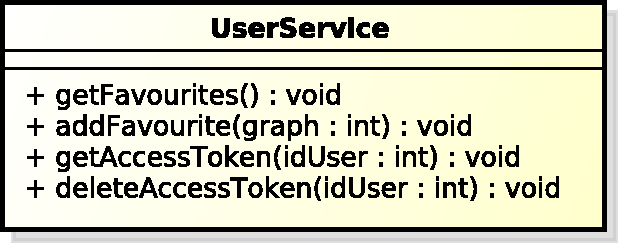
\includegraphics[scale=0.7]{./images/client/classes/model/user_service.pdf}}
				\caption{Classe - client::model::services::RadarChartCreator}
			\end{figure}
			\begin{itemize}
				\item \textbf{Descrizione}: è la classe che gestisce il recupero e la modifica di dati utente relativi a sé stessi;
				\item \textbf{Utilizzo}: i suoi metodi vengono invocati quando un utente accede alla pagina dei propri dati personali;
				\item \textbf{Relazioni con altre classi}:
					\begin{itemize}
						\item client::model::data::UserModel
						\item client::model::services::ManagerDataExpirationDate
						\item client::controller::user::SettingsCtrl
					\end{itemize}
				\item \textbf{Attributi}: N/A
				\item \textbf{Metodi}:
				\begin{itemize}
					\item \textcolor{forestgreen}{\texttt{+ getFavourites()}}
					\begin{description}
						\item \textbf{Descrizione}: metodo che restituisce la lista dei grafici favoriti. 
					\end{description}
					\item \textcolor{forestgreen}{\texttt{+ addFavourite(graph)}}
					\begin{description}
						\item \textbf{Descrizione}: metodo per aggiungere ai favoriti un grafico. Riceve un JSON nella forma:
								\begin{verbatim}
									{
									    metrics: array di MetricModel,
									    kind: JSON nella forma descritta da TypeView
									}
								\end{verbatim}  
					\end{description}
					\item \textcolor{forestgreen}{\texttt{+ getAccessToken(idUser)}}
					\begin{description}
						\item \textbf{Descrizione}: metodo per generare un token di accesso alle api. Prende come argomento l'id dell'utente per cui generare il token. Questo metodo chiama il servizio \textbf{DataManagerService} per effettuare il collegamento con il \textbf{server}, il quale genererà il token secondo lo schema previsto e lo invierà in risposta al client associandolo alle informazioni dell'utente;
					\end{description}
					\item \textcolor{forestgreen}{\texttt{+ deleteAccessToken(idUser)}}
					\begin{description}
						\item \textbf{Descrizione}: metodo che elimina il token generato per l'utente identificato da idUser.
					\end{description}
					
				\end{itemize}
			\end{itemize}
		% subparagraph client_model_services_userservice (end)

		\subparagraph{client::model::services::UserAdminService} % (fold)
		\label{subp:client_model_services_useradminservice}
		\begin{figure}[htbp]
				\centering
				\centerline{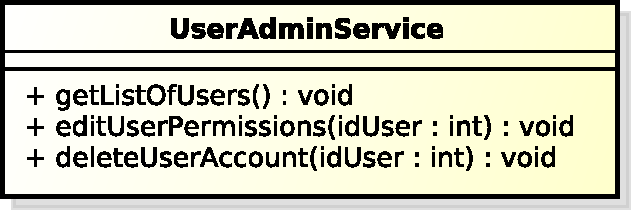
\includegraphics[scale=0.7]{./images/client/classes/model/user_admin_service.pdf}}
				\caption{Classe - client::model::services::RadarChartCreator}
			\end{figure}
			\begin{itemize}
				\item \textbf{Descrizione}: è la classe che oltre a gestire ciò che è gestito dalla sua classe padre si occupa del recupero e della modifica di dati di utenti, inclusa l'eliminazione di un utente e il cambiare i suoi permessi;
				\item \textbf{Utilizzo}: i suoi metodi vengono invocati quando un utente amministratore agisce su dati relativi ad utenti da una pagina non accessibile agli utenti non amministratori;
				\item \textbf{Classi ereditate}:
					\begin{itemize}
						\item client::model::services::UserService
					\end{itemize}
				\item \textbf{Relazioni con altre classi}:
					\begin{itemize}
						\item client::model::data::UserModel
						\item client::model::services::ManagerDataExpirationDate
						\item client::controller::user::UserConfigCtrl
					\end{itemize}
				\item \textbf{Attributi}: N/A
				\item \textbf{Metodi}:
				\item \textcolor{forestgreen}{\texttt{+ getListOfUsers()}}
					\begin{description}
						\item \textbf{Descrizione}: metodo per ottenere la lista degli utenti.
					\end{description}
					\item \textcolor{forestgreen}{\texttt{+ editUserPermissions(idUser)}}
					\begin{description}
						\item \textbf{Descrizione}: metodo per cambiare i permessi di un utente.
					\end{description}
					\item \textcolor{forestgreen}{\texttt{+ deleteUserAccount(idUser)}}
					\begin{description}
						\item \textbf{Descrizione}: metodo per eliminare un utente.
					\end{description}
				\end{itemize}
		% subparagraph client_model_services_useradminservice (end)

		\subparagraph{client::model::services::ChartCreator} % (fold)
		\label{subp:chartcreator}
			\begin{figure}[htbp]
				\centering
				\centerline{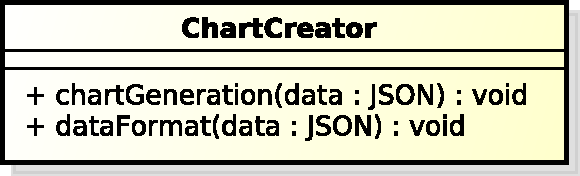
\includegraphics[scale=0.7]{./images/client/classes/model/chart_creator.pdf}}
				\caption{Classe - client::model::services::ChartCreator}
			\end{figure}
			\begin{itemize}
				\item \textbf{Descrizione}: è una classe astratta che descrive il codice comune delle classi che generano un grafico, secondo il pattern \emph{template method};
				\item \textbf{Utilizzo}: i suoi metodi vengono invocati dalle classi figlie nella creazione di grafici;
				\item \textbf{Relazioni con altre classi}:
					\begin{itemize}
						\item client::model::data::ViewTypeModel
						\item client::model::services::LineChartCreator
						\item client::model::services::BarChartCreator
						\item client::model::services::MapChartCreator
						\item client::model::services::PieChartCreator
						\item client::model::services::RadarChartCreator
						\item client::controller::user::ChartsCtrl
						\item client::controller::user::CompareCtrl
					\end{itemize}
				\item \textbf{Attributi}: N/A
				\item \textbf{Metodi}: 
					\begin{itemize}
						\item \textcolor{forestgreen}{\texttt{+ chartGeneration(data)}}
						\begin{description}
							\item \textbf{Descrizione}: metodo che definisce le operazioni comuni di generazione di un grafico. Riceve com argomento un JSON nella forma:
							\begin{verbatim}
									{
									    desc: "descrizione del grafico",
									    datasets: array di array di numeri,
									    labels: array di stringhe,
									    grouping: "weekly/monthly/year/per post" 
									}
								\end{verbatim}  
						\end{description}
						\item \textcolor{forestgreen}{\texttt{+ dataFormat(data)}}
						\begin{description}
							\item \textbf{Descrizione}: metodo per portare i dati nel formato corretto per lo specifico tipo di grafico. Riceve un JSON nella forma descritta per il metodo chartGeneration.
						\end{description}

					\end{itemize}
			\end{itemize}
		% subparagraph chartcreator (end)

		\subparagraph{client::model::services::LineChartCreator} % (fold)
		\label{subp:linechartcreator}
			\begin{figure}[htbp]
				\centering
				\centerline{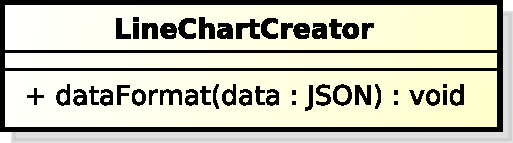
\includegraphics[scale=0.7]{./images/client/classes/model/line_chart_creator.pdf}}
				\caption{Classe - client::model::services::LineChartCreator}
			\end{figure}
			\begin{itemize}
				\item \textbf{Descrizione}: la classe contiene i metodi per la creazione di un Line Chart;
				\item \textbf{Utilizzo}: i suoi metodi vengono invocati quando si vuole creare un Line Chart;
				\item \textbf{Classi ereditate}:
					\begin{itemize}
						\item client::model::services::ChartCreator
					\end{itemize}
				\item \textbf{Relazioni con altre classi}:
					\begin{itemize}
						\item client::controller::user::ChartsCtrl
						\item client::controller::user::CompareCtrl
					\end{itemize}
				\item \textbf{Attributi}: N/A
				\item \textbf{Metodi}: 
					\item \textcolor{forestgreen}{\texttt{+ dataFormat(data)}}
						\begin{description}
							\item \textbf{Descrizione}: metodo per portare i dati nel formato corretto per un line chart. Riceve un JSON nella forma descritta per il metodo chartGeneration.
						\end{description}
			\end{itemize}
		% subparagraph linechartcreator (end)


		\subparagraph{client::model::services::BarChartCreator} % (fold)
		\label{subp:barchartcreator}
			\begin{figure}[htbp]
				\centering
				\centerline{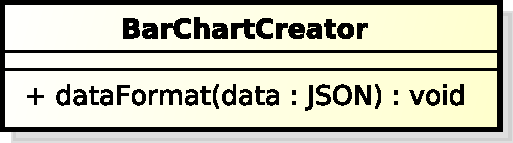
\includegraphics[scale=0.7]{./images/client/classes/model/bar_chart_creator.pdf}}
				\caption{Classe - client::model::services::BarChartCreator}
			\end{figure}
			\begin{itemize}
				\item \textbf{Descrizione}: la classe contiene i metodi per la creazione di un Bar Chart;
				\item \textbf{Utilizzo}: i suoi metodi vengono invocati quando si vuole creare un Bar Chart;
				\item \textbf{Classi ereditate}:
					\begin{itemize}
						\item client::model::services::ChartCreator
					\end{itemize}
				\item \textbf{Relazioni con altre classi}:
					\begin{itemize}
						\item client::controller::user::ChartsCtrl
						\item client::controller::user::CompareCtrl
					\end{itemize}
				\item \textbf{Attributi}: N/A
				\item \textbf{Metodi}: 
					\item \textcolor{forestgreen}{\texttt{+ dataFormat(data)}}
						\begin{description}
							\item \textbf{Descrizione}: metodo per portare i dati nel formato corretto per un bar chart. Riceve un JSON nella forma descritta per il metodo chartGeneration.
						\end{description}
			\end{itemize}
		% subparagraph barchartcreator (end)

		\subparagraph{client::model::services::PieChartCreator} % (fold)
		\label{subp:piechartcreator}
			\begin{figure}[htbp]
				\centering
				\centerline{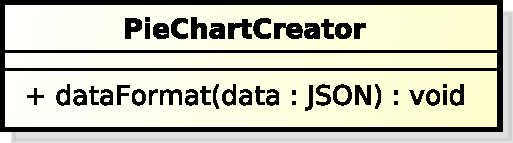
\includegraphics[scale=0.7]{./images/client/classes/model/pie_chart_creator.pdf}}
				\caption{Classe - client::model::services::PieChartCreator}
			\end{figure}
			\begin{itemize}
				\item \textbf{Descrizione}: la classe contiene i metodi per la creazione di un Pie Chart;
				\item \textbf{Utilizzo}: i suoi metodi vengono invocati quando si vuole creare un Pie Chart;
				\item \textbf{Classi ereditate}:
					\begin{itemize}
						\item client::model::services::ChartCreator
					\end{itemize}
				\item \textbf{Relazioni con altre classi}:
					\begin{itemize}
						\item client::controller::user::ChartsCtrl
						\item client::controller::user::CompareCtrl
					\end{itemize}
				\item \textbf{Attributi}: N/A
				\item \textbf{Metodi}: 
					\item \textcolor{forestgreen}{\texttt{+ dataFormat(data)}}
						\begin{description}
							\item \textbf{Descrizione}: metodo per portare i dati nel formato corretto per un pie chart. Riceve un JSON nella forma descritta per il metodo chartGeneration.
						\end{description}
			\end{itemize}
		% subparagraph piechartcreator (end)

		\subparagraph{client::model::services::MapChartCreator} % (fold)
		\label{subp:mapchartcreator}
			\begin{figure}[htbp]
				\centering
				\centerline{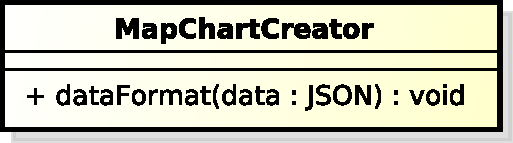
\includegraphics[scale=0.7]{./images/client/classes/model/map_chart_creator.pdf}}
				\caption{Classe - client::model::services::MapChartCreator}
			\end{figure}
			\begin{itemize}
				\item \textbf{Descrizione}: la classe contiene i metodi per la creazione di un Map Chart;
				\item \textbf{Utilizzo}: i suoi metodi vengono invocati quando si vuole creare un Map Chart;
				\item \textbf{Classi ereditate}:
					\begin{itemize}
						\item client::model::services::ChartCreator
					\end{itemize}
				\item \textbf{Relazioni con altre classi}:
					\begin{itemize}
						\item client::controller::user::ChartsCtrl
						\item client::controller::user::CompareCtrl
					\end{itemize}
				\item \textbf{Attributi}: N/A
				\item \textbf{Metodi}: 
					\item \textcolor{forestgreen}{\texttt{+ dataFormat(data)}}
						\begin{description}
							\item \textbf{Descrizione}: metodo per portare i dati nel formato corretto per un map chart. Riceve un JSON nella forma descritta per il metodo chartGeneration.
						\end{description}
			\end{itemize}
		% subparagraph mapchartcreator (end)

		\subparagraph{client::model::services::RadarChartCreator} % (fold)
		\label{subp:radarchartcreator}
			\begin{figure}[htbp]
				\centering
				\centerline{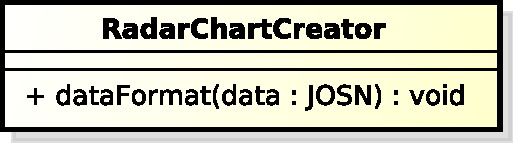
\includegraphics[scale=0.7]{./images/client/classes/model/radar_chart_creator.pdf}}
				\caption{Classe - client::model::services::RadarChartCreator}
			\end{figure}
			\begin{itemize}
				\item \textbf{Descrizione}: la classe contiene i metodi per la creazione di un Radar Chart;
				\item \textbf{Utilizzo}: i suoi metodi vengono invocati quando si vuole creare un Radar Chart;
				\item \textbf{Classi ereditate}:
					\begin{itemize}
						\item client::model::services::ChartCreator
					\end{itemize}
				\item \textbf{Relazioni con altre classi}:
					\begin{itemize}
						\item client::controller::user::ChartsCtrl
						\item client::controller::user::CompareCtrl
					\end{itemize}
				\item \textbf{Attributi}: N/A
				\item \textbf{Metodi}: 
					\item \textcolor{forestgreen}{\texttt{+ dataFormat(data)}}
						\begin{description}
							\item \textbf{Descrizione}: metodo per portare i dati nel formato corretto per un radar chart. Riceve un JSON nella forma descritta per il metodo chartGeneration.
						\end{description}
			\end{itemize}
		% subparagraph radarchartcreator (end)

		\subparagraph{client::model::services::DataManagerService} % (fold)
		\label{subp:radarchartcreator}
		\begin{figure}[htbp]
				\centering
				\centerline{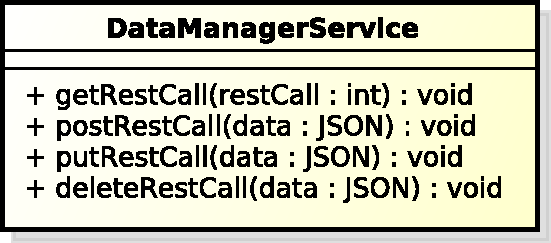
\includegraphics[scale=0.7]{./images/client/classes/model/data_manager_service.pdf}}
				\caption{Classe - client::model::services::RadarChartCreator}
			\end{figure}
			\begin{itemize}
				\item \textbf{Descrizione}: questa classe gestisce l'inoltro di chiamate REST al server. Se si tratta di chiamate Get controlla se i dati che vengono richiesti sono già presenti in locale o se devono essere richiesti al server. In particolare, li richiede al server solo se questi sono assenti o se sono l'ultima volta che sono stati chiesti al server è passata da troppo tempo;
				\item \textbf{Utilizzo}: i suoi metodi vengono invocati dalle classi che desiderano fare richieste al server;
				\item \textbf{Relazioni con altre classi}:
					\begin{itemize}
						\item client::model::services::RecipeService
						\item client::model::services::RecipeAdminService
						\item client::model::services::UserService
						\item client::model::services::UserAdminService
					\end{itemize}
				\item \textbf{Attributi}: N/A
				\item \textbf{Metodi}: 
				\begin{itemize}
					\item \textcolor{forestgreen}{\texttt{+ getRestCall(restCall)}}
						\begin{description}
							\item \textbf{Descrizione}: metodo che controlla se i risultati di una chiamata rest passata per argomento sono presenti in locale, e se non lo sono chiama il server restituendo comunque i dati richiesti.
						\end{description}
					\item \textcolor{forestgreen}{\texttt{+ postRestCall(data)}}
						\begin{description}
							\item \textbf{Descrizione}: metodo per inviare chiamate Rest di tipo post al Server. Prima di aggiornare i dati sul Server aggiorna prima i dati eventualmente presenti in locale.
						\end{description}
					\item \textcolor{forestgreen}{\texttt{+ putRestCall(data)}}
						\begin{description}
							\item \textbf{Descrizione}: metodo per inviare chiamate Rest di tipo put al Server. Prima di aggiornare i dati sul Server aggiorna prima i dati eventualmente presenti in locale.
						\end{description}
					\item \textcolor{forestgreen}{\texttt{+ deleteRestCall(data)}}
						\begin{description}
							\item \textbf{Descrizione}: metodo per inviare chiamate Rest di tipo delete al Server. Prima di aggiornare i dati sul Server aggiorna prima i dati eventualmente presenti in locale.
						\end{description}
				\end{itemize}		
			\end{itemize}
		% subparagraph managerdataexpirationdate (end)

% subsubsection bdsm_app_client_model_services (end)
